\section{Sphere Packing Fundamentals}

This section is divided into two subsections. The first defines fundamental notions about general sphere packings, lattice packings and periodic packings. The third subsection studies the sphere packing of our interest: the $E_8$ lattice packing.

\subsection{The General Theory of Sphere Packings}

We begin by defining a sphere packing.

\begin{boxdefinition}[Sphere Packing]
    Fix $d \in \N$ and $X \subset \R^d$. Assume that there exists a real number $r > 0$, known as the \textbf{separation radius}, such that
    \begin{align*}
        \norm{x - y} \geq r
    \end{align*}
    for all distinct $x, y \in X$. We define the \textbf{sphere packing with centres at $X$} to be
    \begin{align*}
        \Pa(X) := \bigcup_{x \in X} B_d(x, r)
    \end{align*}
\end{boxdefinition}

The density of a sphere packing is the limit superior of an indicator of how much of a bounded region of space a sphere packing covers.

\begin{boxdefinition}[Density]\label{Ch2:Def:Density}
    Let $\Pa$ be a sphere packing. Define the \textbf{density} of $\Pa$ to be
    \begin{align*}
        \Delta(\Pa) := \limsup_{R \to \infty}\frac{\Volof{\Pa \cap B_d(0, R)}}{\Volof{B_d(0, R)}}
    \end{align*}
\end{boxdefinition}

As one might expect, finite density and density are invariant under scaling. We now define lattice and periodic packings.

\begin{boxdefinition}[Lattice and Periodic Sphere Packings]
    A \textbf{lattice} in a Euclidean space $\R^n$ is a discrete $\Z$-submodule of $\R^n$ such that its $\R$-span contains every element in $\R^n$. We say a sphere packing $\Pa(X)$ is
    \begin{enumerate}
        \item a lattice packing if $X$ is a lattice.
        \item $\Lambda$-periodic if for all $\lambda \in \Lambda$ and $x \in X$, we have that $\lambda + x \in X$, where $\Lambda$ is a lattice.
    \end{enumerate}
\end{boxdefinition}

The periodicity property of a periodic sphere packing can be exploited to derive a more convenient formula for its density.

\begin{boxproposition}\label{Ch2:Prop:Periodic_Density}
    Let $\Pa(X)$ be a sphere packing with centres at $X \subset \R^d$ and separation $r$ that is periodic with respect to some lattice $\Lambda \subset \R^d$. We have that
    \begin{align}
        \Delta_{\Pa(X)} = \abs{\quotient{X}{\Lambda}} \frac{\Volof{B_d\of{0, \frac{r}{2}}}}{\Volof{\quotient{\R^d}{\Lambda}}}
        \label{Ch2:Eq:Periodic_Density}
    \end{align}
    where $\abs{\quotient{X}{\Lambda}}$ is the number of orbits of the additive $\Lambda$-action on $X$ and $\Volof{\quotient{\R^d}{\Lambda}}$ is the volume of the fundamental domain of the $\Lambda$-action on $\R^d$.
\end{boxproposition}

Interestingly, one can show that the supremum of densities taken over all sphere packings in $\R^n$ is the same as the supremum taken over all periodic packings in $\R^n$. A proof can be found in \cite[Appendix A]{CohnElkies}. We denote this quantity by $\Delta_n$, $n$ being the dimension of the ambient space.

We will end by defining dual lattices. Viewing a lattice in $\R^d$ as a free $\Z$-submodule of $\R^d$, we can view its dual lattice as the corresponding submodule of $\parenth{\R^d}^*$. We offer a slightly more convenient definition.

\begin{boxdefinition}[Dual Lattice]\label{Ch2:Def:Dual_Lattice}
    Fix $d > 0$ and let $\Lambda \subset \R^d$ be a lattice. We define the \textbf{dual lattice} of $\Lambda$ to be
    \begin{align*}
        \Lambda^* := \setst{y \in \R^d}{\cycl{x, y} \in \Z \text{ for all } x \in \Lambda}
    \end{align*}
\end{boxdefinition}

We are now ready to discuss a special sphere packing in $\R^8$: the $E_8$ sphere packing.

\subsection{The $E_8$ Lattice Packing}\label{Ch2:Subsec:E8}

It is quite remarkable that $E_8$ should show up when discussing sphere packings. At its core, $E_8$ is an irreducible root system. It shows up in the classification of important classes of objects like irreducible Coxeter groups, crystallographic Coxeter groups, and semi-simple Lie algebras over $\C$. $E_8$ is not a classical root system but an \textit{exceptional} root system, meaning that the geometric properties of its roots cannot be found in irreducible root systems in all dimensions.

\begin{wrapfigure}[19]{r}{0.5\linewidth}
    \centering
    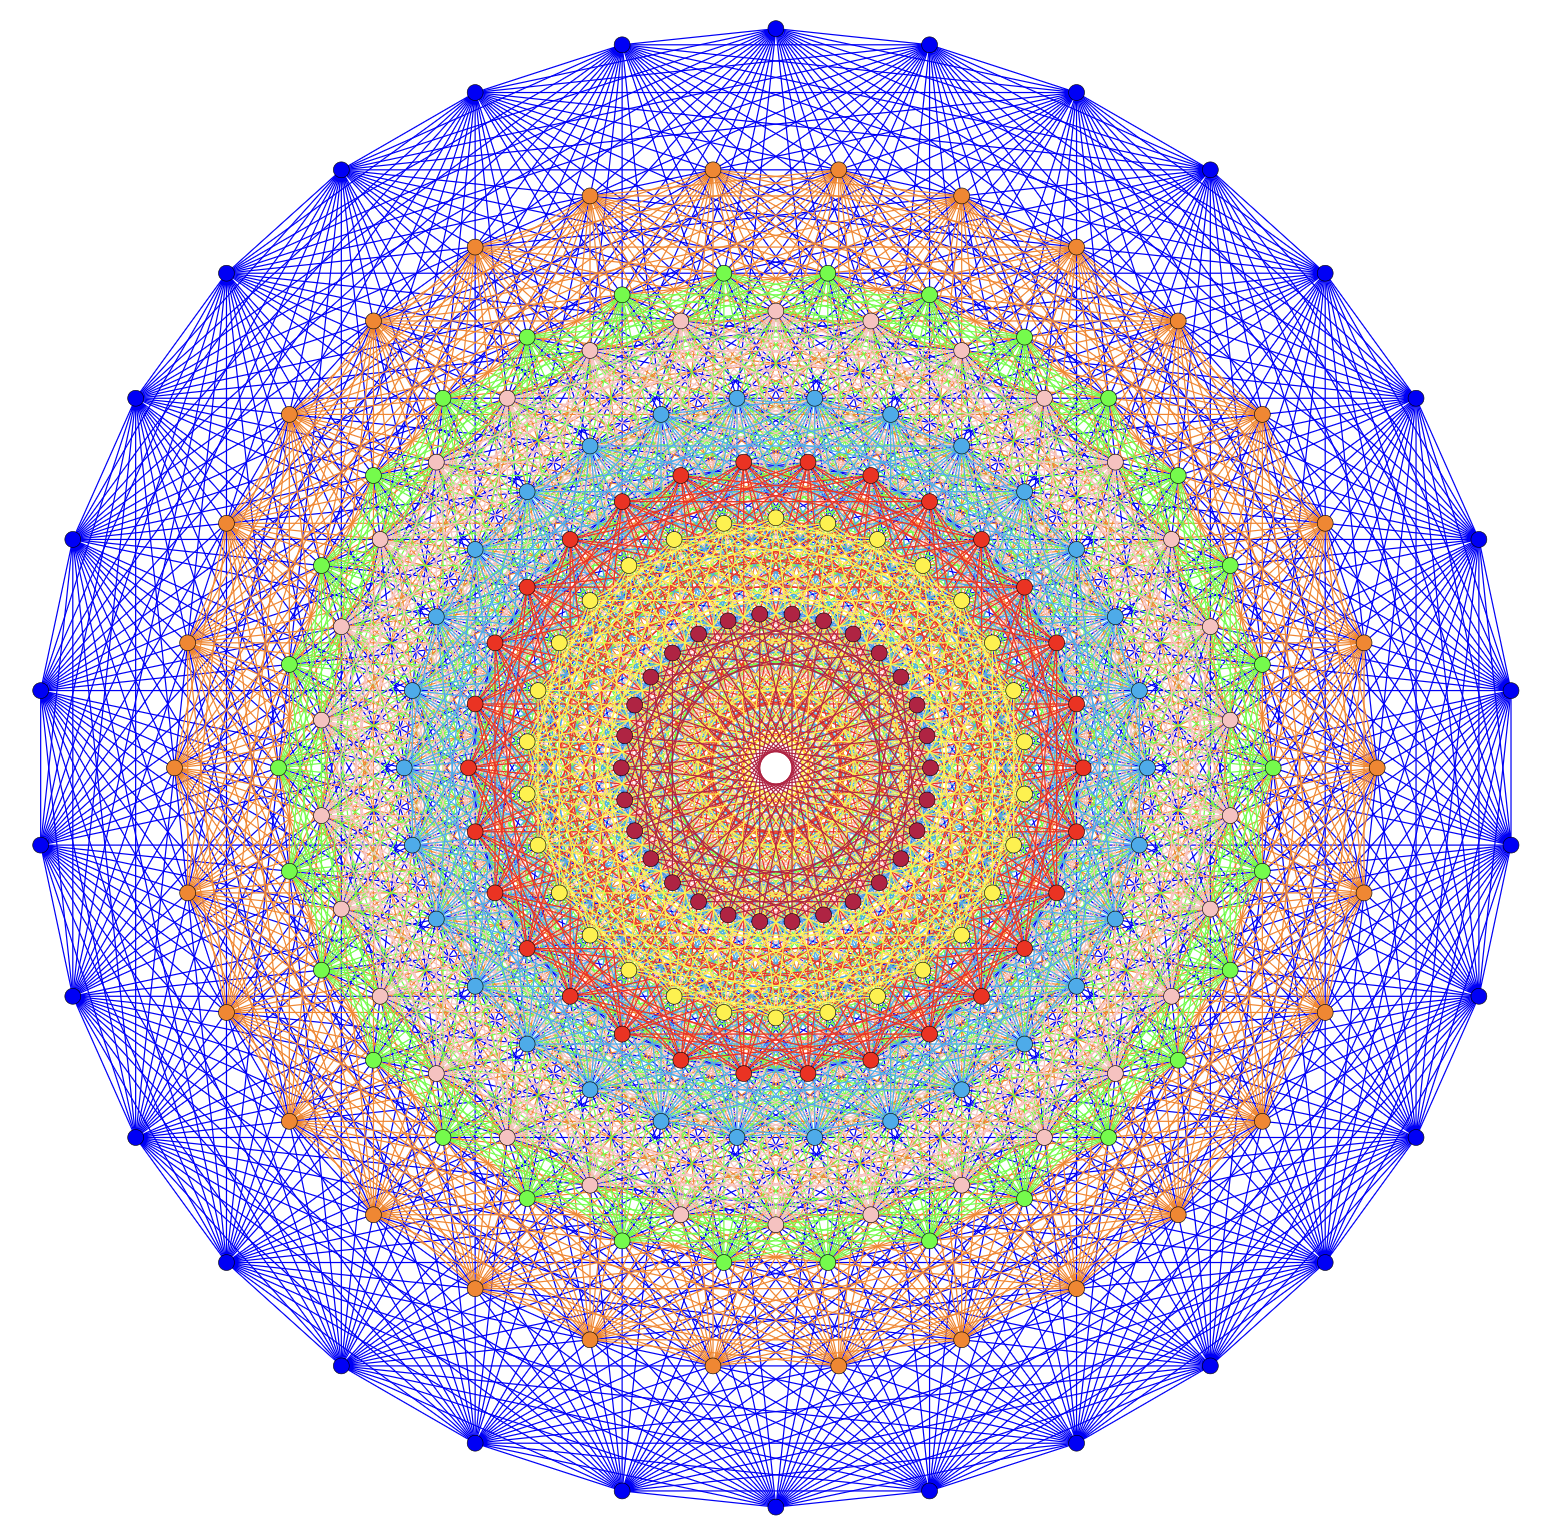
\includegraphics[width=0.98\linewidth]{Chapters/2_Dimension_8/Images/Gorbe_E8.png}
    \caption{The Coxeter projection of the $E_8$ root system. \cite{Gorbe_E8}}
    \label{Ch2:Fig:Gorbe_E8}
\end{wrapfigure}

The $E_8$ root system consists of $240$ vectors in $\R^8$ that are permuted by a certain finite subgroup of the $8$-dimensional orthogonal group. This group is sometimes referred to as the $E_8$ Coxeter group or as the Weyl group of the $E_8$ lattice. These roots can be divided into $8$ orbits, each of which corresponds to one of the `layers' of concentric circles in \Cref{Ch2:Fig:Gorbe_E8}. The dots in the figure correspond to projections of the roots onto a plane on which a specific type of element of the Coxeter group, known as a Coxeter element, acts as a rotation. This visualisation offers a convenient---and aesthetically pleasing---means of visualising this collection of $8$-dimensional vectors and appreciating some of its symmetry.

The $E_8$ lattice is characterised in many ways. One is as the $\Z$-span of the so-called \textit{simple roots} of the $E_8$ root system, the simple roots being a distinguished basis of $\R^8$ that is contained in the $E_8$ root system. Another is that up to isomorphism, the $E_8$ lattice is the unique positive-definite, even, unimodular lattice in $\R^8$. We instead give the following explicit definition of the $E_8$ lattice, which we attempted to reconcile with the `\verb|Zspan|' characterisation in Lean.

\begin{boxdefinition}[The $E_8$ Lattice]\label{Ch2:Def:E8_Lattice}
    The $E_8$ lattice consists of all vectors in $\R^8$ such that either all coordinates are integers or all coordinates are half-integers and the sum of all coordinates is even. That is,
    \begin{align*}
        \Lambda_8 := \setst{\parenth{x_1, \ldots, x_8} \in \Z^8 \cup \parenth{\Z + \frac{1}{2}}^8}{\sum_{i=1}^{8} x_i \equiv 0 \pmod{2}}
    \end{align*}
\end{boxdefinition}

For the construction of the magic function, we will primarily rely on the following facts.
\begin{boxproposition}[Properties of the $E_8$ Lattice]\label{Ch2:Prop:E8_Properties}
    The following are true of the $E_8$ lattice.
    \begin{enumerate}
        \item For all $x, y \in \Lambda_8$, $\norm{x - y} \geq \sqrt{2}$.
        \item The density of the sphere packing centred at points in $\Lambda_8$ with separation $\sqrt{2}$ is
        \begin{align*}
            \frac{\pi^4}{384} \approx 0.2536695
        \end{align*}
        \item The elements of $\Lambda_8$ all have norm $\sqrt{2n}$ for some $n \in \N$.
        \item The dual lattice of $\Lambda_8$ is $\Lambda_8$.
        \item The covolume of $\Lambda_8$ is $1$. Ie, $\Volof{\quotient{\R^8}{\Lambda_8}} = 1$.
    \end{enumerate}
\end{boxproposition}

The sphere packing to which we refer in the second point of the above theorem is precisely the $E_8$ sphere packing. We are now ready to examine Cohn and Elkies's groundbreaking intermediate result that Viazovska uses to construct her Magic Function.
